\chapter{User Guide}

\section{Introduction}

The \textsc{Visual Service Design Tool} is an Eclipse based graphical editor for designing, validating and exporting Business Process Diagrams based on the Business Process Modeling Notation.

\subsection{ Features }

\begin{itemize}
\item as a plugin for the popular Eclipse Framework the editor is platform independent, easy to install and has a familiar look and feel
\item using the Eclipse Graphical Modeling Framework and a modular structure consisting of several sub-plugins the editor can easily be modifies and enriched with new features, e.g. additional custom actions or export wizards
\item it provides all the basic editing features like undo and redo for each editing operation, zooming, printing diagrams to various image formats, and many more
\item the editor is based on the BPMN specification, which is easy to understand by business men and formal enough for being exported to executable languages
\item the diagrams drawn with the editor can be validated according to the constraints given in the BPMN specification
\item diagrams valid to the specification can be exported to executable languages, such as WS-BPEL and JIAC
\end{itemize}



\subsection{Components and Dependencies}

The Visual Service Design Tool consists of several features:

\begin{itemize}
\item \texttt{VSDT} This feature is holding the plugins for the visual editor.
\item \texttt{BpmnExport} This feature is holding plugins needed for the transformation, like a reference model and a transformation system.
\item \texttt{Bpmn2Bpel} This feature is holding the plugins needed for the export to BPEL, such as a wizard, transformation rules and a visitor
\item \texttt{Bpmn2Jiac} This feature is holding the plugins needed for the export to JIAC IV, such as a wizard, transformation rules and a visitor
\end{itemize}

Since the editor is based on the Graphical Modeling Framework, the GMF PlugIn is required for the execution as well as all of its prerequisites.


\subsection{Installation}

\paragraph*{Installing Eclipse and GMF}

To use the Visual Service Design Tool you need the Eclipse IDE which can be found at \url{http://www.eclipse.org}. Further you will need the Graphical Modeling Framework (GMF). For the 2.2.x release you will need Eclipse 3.3 and GMF 2\footnote{note that GMF itself will have some more dependencies}. You can get GMF at \url{http://www.eclipse.org/gmf}. However, it is recommended to use the Eclipse Update feature. Make sure you are allowed to write in the Eclipse program folder. In Eclipse, select \emph{Help} from the menu, then \emph{Software Updates} and \emph{Find and Install...}. Search for \emph{new features to install} using the \emph{Europa Discovery Site} and select the Graphical Modeling Framework from the list. Further, click on \emph{Select Required} to automatically check all required features, like EMF and GEF, from the list. Finally, continue through the installation process and restart Eclipse. If the installation was successfull the new features should appear in the \emph{Manage Configuration} dialog which can be found in the same menu.

\paragraph*{Installing the Visual Service Design Tool}

Once Eclipse-GMF is set up you can install VSDT. You can find the latest version at the \emph{SerCHo Update Site} \footnote{\url{http://sercho-dev.dai-labor.de/repository/update-site/}}. You can add this site as a \emph{New Remote Site} in the \emph{Find and Install...} dialog (see last section) or download one of the archives. If the archive contains a site.xml you can add the archive as a \emph{New Archived Site} and use the update feature to install the plugins in the archive, otherwise you can manually extract the archive and merge the contained \verb|feature| and \verb|plugin| directories with the ones found in your Eclipse program directory.


\subsection{The Eclipse Environment}

This section will briefly introduce those parts of the Eclipse GUI that are relevant for the work with the Visual Service Design Tool.

\begin{figure}[htp]
\centering
\includegraphics[width=.75\textwidth]{figures/screens/gui.png}
\caption[Snapshot of Eclipse GUI]{A snapshot of the Eclipse GUI.}
\label{fig:gui}
\end{figure}

\paragraph*{The Project Explorer}
Here the user can manage his projects and create and delete files.  Note that Eclipse provides different similar views for managing files, e.g. the Navigator or the Package Explorer. However, only the Project Explorer is supported by the GMF, which allows to expand a Business Process Diagram file in the Project Explorer and inspect it's elements without actually opening it.

\paragraph*{The Editor View}
The editor window is shown automatically when opening a file in the Project Explorer. Depending on the PlugIns currently installed this can be a plain text editor, a browser, an elaborate code editor or some sort of graphical editor. For the \textsc{Visual Service Design Tool} there are two editors available. The visual editor is for drawing the business process diagrams figures and connections. Still there are non-graphical elements which can't be represented with nodes and connections. For managing and editing those elements there is a tree editor which hierarchically lists all the elements.

\subparagraph*{The Graphical Editor}
This editor is opened when the diagram file is clicked. On the right side there is a palette with all the nodes and connections. Not all of the nodes can be placed directly on the canvas, e.g. the various Flow Objects can only be placed within a lane, with again must be placed inside a pool.

\subparagraph*{The Tree Editor}
The tree editor is sometimes needed for managing and editing those parts of the Business Process Diagram that do not have a graphical representation, e.g. Assignments, Participants, or Messages. Note that the tree editor is more powerful than the graphical editor, and the diagram might be invalidated when doing certain operations in the tree editor. Where ever possible the graphical editor should be used. The tabs at the bottom line of the editor provide some selection-sensitive views on the tree. You can select some element in the outline (see below) and the tabs will show e.g. this elements parents or children in different ways.

\paragraph*{The Properties View}
Although some attributes, like an element's name, can be edited in the editor view as well, for most other attributes the properties view will be needed. Here all the attributes relevant for the user can be seen and edited. All changes done in the properties view can be undone and redone; the editor is updated immediately.

\paragraph*{The Outline}
This view provides a short outline of the current editor's content. In case of a graphical editor this could be a miniature view of the entire diagram, in case of a tree editor an additional tree editor for easier navigation. 

\paragraph*{The Problem View}
This view lists all the problems that eventually have been found in the model, subdivided in errors and warnings. By double-clicking one of the items the editor will focus on the element the problem occurred on.

\paragraph*{The Error Log}
Other than the Problem View the Error Log will log problems that happened with the editor itself. So if you should encounter strange behavior or in case the editor should crash you can check here for the reason and send in an error report.



\section{Basic Tutorial}

%%%%%%%%%%%%%%%%%%%%%%%%%%%%%%%%%%
% tutorial an konkretem beispiel?
%%%%%%%%%%%%%%%%%%%%%%%%%%%%%%%%%%

In this section we will explain the basic steps how to create a simple Business Process Diagram.

\begin{enumerate}

\item First a \textbf{new Project} and a Diagram have to be created. To do so select \emph{ New $\rightarrow$ Project $\rightarrow$ General $\rightarrow$ Project } in the menu bar and then \emph{ New $\rightarrow$ Visual Service Design Tool $\rightarrow$ BPMN Diagram }. Open the Project Explorer to see the newly created Project and within the project two files. The first file is for the pure model data and the other one holds the layout information for the diagram.

\emph{Note} that both files are stored in XML format and can be edited with a text editor, too. However, you should do so only to fix a broken file. The diagram file can be recreated from the model file by right clicking it and choosing to initialize the diagram file.

\item \textbf{Open both files} by double clicking them. The model file will be opened with the tree editor, the diagram file with the graphical editor. For now, ignore the model file.

\item In the graphical editor select a \textbf{Pool} from the palette. Move the mouse to the canvas. Note that the mouse cursor changes where you can create a Pool. Push the mouse button and drag it to the lower right to create a large Pool. Enter a name for the Pool when you are prompted to.

\item Select the \textbf{Lane} element from the palette and click somewhere on the Pool. The Lane will be created in the top of the Pool, independent from where you click. According to the BPMN specification the first Lane will be invisible (faded out in the editor), so don't be confused.

Create a second Lane on the Pool and both Lanes will be visible. Note that the Lanes can not be resized or moved. They will adapt automatically to the elements within. You can right-click the Pool and select \emph{Auto Size} from the format menu and the Pool will automatically adapt it's size to the Lane's size, too.

\item Let's create some \textbf{Flow Objects} inside the Lanes. Hover the mouse over one of the Lanes until you can see a miniature palette floating over he Lane. Select the Start Event icon and name it (see figure \ref{fig:tut_1}). Create an Activity and an End Event. Try different ways, e.g. from the palette or by hovering the mouse.

\begin{figure}[htp]
\centering
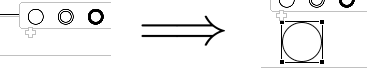
\includegraphics[width=.5\textwidth]{figures/tut/tut_1.png}
\caption{Creating a Start Event}
\label{fig:tut_1}
\end{figure}


Select the Sequence Flow icon from the palette and connect the Start Event with the Activity and the Activity with the End Event by pressing the mouse button on the source and dragging it to the target. When connecting the Activity be sure to aim for the label. If you hit the Activity's compartment you can not create a connection. You can change the routing style from the toolbar or add bendpoints to a connection by dragging it.

\item Now select the \textbf{Message Flow} icon from the palette. Select the End Event as source and draw the Message Flow to some point beneath the Pool and select to create a new Pool element there (see figure \ref{fig:tut_2}). Expand the Pool to the entire width of the diagram.

\begin{figure}[htp]
\centering
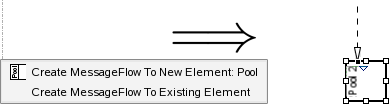
\includegraphics[width=.5\textwidth]{figures/tut/tut_2.png}
\caption{Creating a Message Flow to a new Pool}
\label{fig:tut_2}
\end{figure}

Right-Click both Pools and select \emph{Initialize Participant} from the BPMN menu. Take a look at the properties view to see the newly created Participant elements. Now right-click the Message Flow and select \emph{Initialize Message} (see figure \ref{fig:tut_3}). Note that the End Event's type changed to \texttt{Message}. A new Message has been created and automatically associated with the Pool's Participants, the Message Flow and the source and target (if possible).

\begin{figure}[htp]
\centering
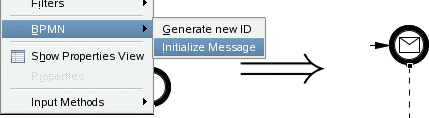
\includegraphics[width=.5\textwidth]{figures/tut/tut_3.png}
\caption{Initializing the Message}
\label{fig:tut_3}
\end{figure}

\item Let's associate a Data Object with the Activity. Hover the mouse over the Activity and select the incoming Arrow. Drag the mouse to some point outside of the Pool and release the mouse button. Select to create an Association to a new Data Object element (see figure \ref{fig:tut_5}). Select the Association and set the Direction Type to \texttt{To} in the properties view (if you dragged the outgoing arrow before select \texttt{From} instead).

\begin{figure}[htp]
\centering
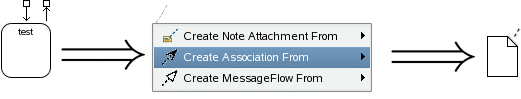
\includegraphics[width=.5\textwidth]{figures/tut/tut_5.png}
\caption{Creating an Association to a new Data Object}
\label{fig:tut_5}
\end{figure}

To complete this step select \emph{BPMN $\rightarrow$ Initialize Input Set} from the Activity's context menu. Notice the new Input Element in the Activity's property sheet (see figure \ref{fig:tut_6}). This Input Set references all the Activity's incoming Data Objects.

\begin{figure}[htp]
\centering
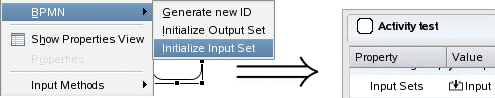
\includegraphics[width=.5\textwidth]{figures/tut/tut_6.png}
\caption{Initializing a new Input Set with the associated Data Object}
\label{fig:tut_6}
\end{figure}

\item Finally select \emph{Validate} from the Diagram menu. You might notice some errors or warnings in your diagram. For now you can ignore these, but for exporting diagrams to executable code there should be no errors left in the diagram.

Save your diagram and change to the tree editor. Here you can inspect the attributes of non-graphical elements like the Message, the End Event's Message Trigger Attribute Set or the Activity's Input Set. By right-clicking the Business Process Diagram element in the tree editor you can create new Supporting Types, e.g. for Messages and Implementations. Note that you might have to close and reopen the graphical editor for changes made in the tree editor to take effect.

\end{enumerate}


\section{How To \dots}

\paragraph*{\dots draw Flow Objects on the Canvas?}
Although such diagrams can be seen in various papers, Flow Objects \emph{can not} be drawn on the canvas. Instead, each Flow Object has to be contained in a Lane, and the Lane has to be in a Pool. However, one Pool per diagram can be set to have an invisible border (you can set more than one Pool to be invisible, but this will result in a validation error).

\paragraph*{\dots draw a Flow Objects in a region of the Pool that is not covered by the Lane?}
Lanes automatically adapt to their contents. If you want to draw a Flow Object in a place that is not covered by the Lane, for instance when starting an alternative path after a Gateway, you can stretch the Lane by inserting the element somewhere in the Lane and gradually moving it toward the Lane's lower border.

\paragraph*{\dots create an Intermediate Event on an Activity's boundary?}
Hover the mouse over the Activity. A miniature palette holding only an Intermediate Event will pop up. select the Intermediate Event and it will be created on the Activity's boundary. You might have to select \emph{Auto Size} from the Activity's context menu if the Event is not placed properly. Select the Event and set its type as you like (see figure \ref{fig:tut_4}).

\begin{figure}[htp]
\centering
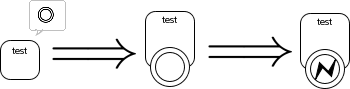
\includegraphics[width=.5\textwidth]{figures/tut/tut_4.png}
\caption{Creation of an Event on an Activity's boundary}
\label{fig:tut_4}
\end{figure}

\paragraph*{\dots draw Artifacts inside of a Pool?}
Contrary to Flow Objects, Artifacts can not be created inside of a Pool. However, you can create the Artifact on the canvas and drag it over the Pool. But remember that the Artifact is \emph{over}, and not \emph{in}, the Pool, so it will not be moved together with the Pool.

\paragraph*{\dots enter a Time Date value?}
This value is expected in quite complex form, because it has to be processed by a parser. The value has to be in the form "yyyy-MM-dd'T'HH:mm:ss.SSSZ", e.g. "2007-02-12T14:53:00.000+0100" for Monday, the 12th of February 2007 at 14:53:00 CET.

\paragraph*{\dots create and edit properties and assignments?}
Right-click on some BPMN element that can hold properties or assignments, e.g. an Activity, a Message Flow (for the message's properties) or a Pool (for the properties of the process). Select \emph{BPMN} $\rightarrow$ \emph{Manage Properties} / \emph{Manage Assignments} and a dialog will appear. Click \emph{New} to create a new element or \emph{Remove} to remove an existing one. To edit the attributes select the element. Its current attributes will appear in the fields below. Enter new values and hit the \emph{Update} button to write these values in the selected property/assignment.

\paragraph*{\dots create and edit other non-graphical Supporting Types?}
For some supporting types, like a Pool's Participant or a Message Flow's Message there are some actions that can be accessed though that element's context menu (in the BPMN group). For managing other non-graphical elements the EMF tree editor has to be used. Save and close the diagram editor and open the model file with the EMF tree editor. Make your changes to the non-graphical elements, save and change back to the diagram editor.
%%%%%%%%%%%%%%%%%%%%%%%%%%%%%
% TODO später ändern!
%%%%%%%%%%%%%%%%%%%%%%%%%%%%
% Note that synchronization of the two editors is not supported yet, so you have to close and reopen the diagram editor each time you make changes in the tree editor, so be careful to save your changes in the diagram editor \emph{before} you change to the tree editor, or you will instantly overwrite the changes done in the tree editor.


\section{Exporting Business Process Diagrams}

Choose the \emph{Export} feature from the \emph{File} menu and select the export wizard of choice in the dialog. Select the model files to export -- not the diagram files! -- and specify a path where to create the target model (see figure \ref{fig:wizard}). For each BPMN model file a folder with the Business Process Diagram's name will be created, holding the generated files together with a log file.

\begin{figure}[ht]
\centering
\includegraphics[width=.5\textwidth]{figures/screens/wizard.png}
\caption[BPMN Export Wizard]{Model selection page of the BPMN to JIAC Export Wizard.}
\label{fig:wizard}
\end{figure}

Note that the diagram has to be in a certain form so it can be successfully transformed. The diagram has to be \emph{structured}, meaning that there must not be blocks or loops with multiple entry or exit points. For each splitting Gateway there has to be a joining Gateway and vice versa. Also note that not each single feature can be taken into account in the transformation yet. For those elements that can not yet be mapped a no-operation element will be created in the target model, such as a \verb|empty| Activity in BPEL or a \verb|logwarn| in JIAC. Be sure to substitute these elements with a proper implementation after the transformation.
